\section{Approximation results for various activation functions}

\subsection{Cosine functions as activation function}
Let us use a simple example to motivate the spectral Barron space. Consider a bounded domain $\Omega\subset \mathbb
R^d$ and a real function $u\in L^1(\Omega)$.
Recall the Fourier transform of $u\in L^1(\mathbb{R})$ in Definition~\ref{def:fourier1} and \ref{def:fourier2}. 
This gives the following integral representation of $u$ in terms of the cosine function
\begin{equation}
 \label{eq:reint}
u(x)=Re\int_{\mathbb{R}^d} e^{2\pi i\omega\cdot x} \hat u(\omega)d\omega
= \int_{\mathbb{R}^d}\cos (2\pi (\omega\cdot x + b(\omega))) |\hat u(\omega)|d\omega,
\end{equation}
where $ \hat u(\omega)= e^{2\pi ib(\omega)}|\hat u(\omega)|$. Let 
\begin{equation}
 \label{eq:2}
g(x, \omega) = \cos(2\pi (\omega\cdot x + b(\omega)))\quad \mbox{ and }\quad 
\rho(\omega)= |\hat u(\omega)| . 
\end{equation}
Thus, 
\begin{equation}
\label{int-rep}
u(x)= \int_{\mathbb{R}^d}g(x,\omega) \rho(\omega)d\omega,   
\end{equation}
If
$$
\int_{\mathbb R^d} |\hat u(\omega)|d\omega <\infty,
$$
then $\|\rho\|_{L^1}<\infty$. By applying the Lemma \ref{lem:sample},
there exist $\omega_i\in \mathbb R^d$
such that
\begin{equation}
  \label{eq:3}
\|u-u_N\|_{0,\Omega}\le N^{-1/2}\|\hat u\|_{L^1(\mathbb R^d)}.  
\end{equation}
where
\begin{equation}\label{cosfn}
u_N(x) = {\|\hat u\|_{L^1(\mathbb R^d)}\over N} \sum_{i=1}^N \cos (2\pi(\omega_i\cdot x + b(\omega_i)))
\end{equation}
More generally, we consider the approximation property in $H^m$-norm.
By \eqref{eq:reint},
\begin{equation} 
\partial^\alpha u(x)= \int_{\mathbb{R}^d} \cos^{|\alpha|}(2\pi (\omega\cdot x + b(\omega)))\omega^\alpha |\hat u(\omega)|d\omega,  \quad \forall\ |\alpha|\le m.
\end{equation}
For any positive integer $m$, let 
\begin{equation} \label{eq:gm}
g_m(x,\omega)= {\cos (2\pi (\omega\cdot x + b(\omega)))\over  (1+ \|\omega\|)^m}\quad \mbox{and}\quad \rho_m(\omega)= (1+ \|\omega\|)^m|\hat u(\omega) |,
\end{equation}
where
$$
\| \rho_m\|_{L^1(\mathbb R^d)}=\int_{\mathbb R^d} (1+ \|\omega\|)^m|\hat u(\omega) | d\omega<\infty.
$$
Then, $\displaystyle u(x)=\int_{\mathbb R^d} g_m(x,\omega)\rho_m d\omega = \| \rho_m\|_{L^1(\mathbb R^d)}\mathbb{E}g_m(x,\omega)$. Define
\begin{equation}
u_N(x) = {\|\rho_m\|_{L^1(\mathbb R^d)}\over N} \sum_{i=1}^N g_m(x,\omega_i)
= {\|\rho_m\|_{L^1(\mathbb R^d)}\over N} \sum_{i=1}^N {\cos (2\pi(\omega_i\cdot x + b(\omega_i)))\over (1+\|\omega_i\|)^m}.
\end{equation}
It holds that 
$$
\partial^\alpha (u(x) - u_N(x))={\|\rho_m\|_{L^1(\mathbb R^d)}\over N}\sum_{i=1}^N \mathbb{E} \partial^\alpha (g_m(x,\omega) -  g_m(x,\omega_i)).
$$
By Lemma \ref{MC},
\begin{align}
\mathbb{E}_N \sum_{|\alpha|\le m}\|\partial^\alpha (u(x) - u_N(x))\|_{0, \Omega}^2 
&\le 
\|\rho_m \|_{L^1(\mathbb R^d)}^2\mathbb{E}_N \sum_{|\alpha|\le m}\frac{1}{N^2}\sum_{i=1}^N \left (\mathbb{E} \partial^\alpha (g_m(x,\omega) -  g_m(x,\omega_i))\right )^2
\\
&\le 
{\|\rho_m \|_{L^1(\mathbb R^d)}^2\over N}  \sum_{|\alpha|\le m}\mathbb{E} \left (\partial^\alpha g_m(x,\omega)\right)^2
\end{align}
Note that the definitions of $g_m$ and $\rho_m$ in \eqref{eq:gm} guarantee that 
$$
|\partial^\alpha g_m(x,\omega)|\le 1.
$$
Thus,
$$
\mathbb{E}_N \sum_{|\alpha|\le m}\|\partial^\alpha (u(x) - u_N(x))\|_{0, \Omega}^2 \lesssim {\|\rho_m \|_{L^1(\mathbb R^d)}^2\over N}.
$$
This implies that there exist
$\omega_i\in \mathbb R^d$ such that
\begin{equation}
\label{cosHm}
\|u-u_N\|_{H^m(\Omega)}\lesssim N^{-1/2}\int_{\mathbb{R}^d} (1+ \|\omega\|)^m|\hat u(\omega) | d\omega.  
\end{equation}


Given $v\in L^2(\Omega)$,   consider all the possible extension $v_E:
\mathbb{R}^d \mapsto \mathbb{R}$ with $v_E |_{\Omega} = v$ and define
the spectral  Barron norm for any $s\ge 1$:
	\begin{equation}\label{barron-norm0}
	\|v\|_{B^{s}(\Omega)} = \inf_{v_E |_{\Omega} = v} \int_{\mathbb{R}^d}(1+\|\omega\|)^s|\hat{v}_E(\omega)|d\omega
	\end{equation}
and  spectral  Barron space
\begin{equation}
  \label{Barron}
	B^{s}(\Omega) = \{v\in L^2(\Omega): \|v\|_{B^{s}(\Omega)}<\infty\}.  
\end{equation}

In summary, we have 
\begin{equation} 
\|u-u_N\|_{H^m(\Omega)}\lesssim N^{-1/2}  \|u\|_{B^{m}(\Omega)},
\end{equation}
where $u_N$ is defined in \eqref{cosfn}.


Specifically, we will consider the problem of approximating a function with bounded Barron norm \eqref{barron-norm0} in the Sobolev space $H^m(\Omega)$. Our first step will be to prove a lemma showing that the Sobolev norm is bounded by the Barron norm.

\begin{lemma}\label{smoothness-lemma}
 Let $m \geq 0$ be an integer and $\Omega\subset \mathbb{R}^d$ a bounded domain. Then for any Schwartz function $v$, we have
 \begin{equation}\label{embend}
 \|v\|_{W^{m,\infty}(\Omega)} \lesssim \|v\|_{{B}^m(\Omega)} \lesssim  \|v\|_{H^{m + {d\over 2}+\epsilon}(\Omega)},
 \end{equation}
 where $\epsilon$ is positive.
\end{lemma}
\begin{proof}
Recall the inverse Fourier transform in Definition \ref{def:fourier1}
$$
v(x)=\int \hat{v}(\omega) e^{2 \pi i\omega \cdot x} d \omega.
$$
For any $|\alpha|\le m$,
$$
|\partial^\alpha v|=|(2\pi)^{|\alpha|}\int \hat{v}(\omega) \omega^\alpha e^{2 \pi i\omega \cdot x} d \omega|\le |(2\pi)^{|\alpha|}\int \hat{v}(\omega) \|\omega\|^\alpha e^{2 \pi i\omega \cdot x} d \omega| \lesssim \|v\|_{B^m(\Omega)},
$$ 
which proves $ \|v\|_{W^{m,\infty}(\Omega)} \lesssim \|v\|_{{B}^m(\Omega)}$.

\iffalse
 Let $\chi$ be a Schwartz function satisfying $\chi(x) = 1$ for $x\in \Omega$. Such a function exists because $\Omega$ is bounded. Let $\alpha$ be any multi-index with $|\alpha|\leq m$. Then we have
 \begin{equation}
  \|D^\alpha v\|_{L^2(\Omega)} \leq \|\chi D^\alpha u\|_{L^2(\mathbb{R}^d)} \leq \|\hat\chi * \widehat{D^\alpha v}\|_{L^2(\mathbb{R}^d)}
 \end{equation}
 Now we use Young's inequality to obtain
 \begin{equation}
  \|\hat\chi * \widehat{D^\alpha v}\|_{L^2(\mathbb{R}^d)} \leq \|\hat\chi\|_{L^2(\mathbb{R}^d)}\|\widehat{D^\alpha v}\|_{L^1(\mathbb{R}^d)} \leq \|\hat\chi\|_{L^2(\mathbb{R}^d)}\|v\|_{\mathcal{B}^m(\Omega)}.
 \end{equation}
 Combining this over all multi-indices $\alpha$, we get
 \begin{equation}
  \|u\|_{H^m(\Omega)} \lesssim \|v\|_{\mathcal{B}^m(\Omega)},
 \end{equation}
 as desired. \fi
 
 A version of the second inequality
  in \eqref{embend} and its proof 
can be found in \cite{barron1993universal}. Below is a proof, by 
definition and Cauchy-Schwarz
  inequality, 
\begin{align}
\|v\|_{B^m(\Omega)} =& \inf_{v_E |_{\Omega} = v} \left(\int_{\mathbb{R}^d}(1+\|\omega\|)^m|\hat{v}_E(\omega)|d\omega \right)^2
\\
\le &  \int_{\mathbb{R}^d}(1+\|\omega\|)^{-d - 2\epsilon}d\omega  \inf_{v_E |_{\Omega} = v} 
\int_{\mathbb{R}^d}(1+\|\omega\|)^{d + 2m + 2\epsilon} |\hat{v}_E(\omega)|^2d\omega  
\\
\lesssim &  \inf_{v_E |_{\Omega} = v} 
\int_{\mathbb{R}^d}(1+\|\omega\|)^{d + 2m + 2\epsilon} |\hat{v}_E(\omega)|^2d\omega  
\lesssim \|v\|_{H^{m + {d\over 2}+\epsilon}(\Omega)}.
\end{align}


\end{proof}



%
\subsection{Cosine functions as activation function}
Let us use a simple example to motivate the spectral Barron space. Consider a bounded domain $\Omega\subset \mathbb
R^d$ and a real function $u\in L^1(\Omega)$.
Recall the Fourier transform of $u\in L^1(\mathbb{R})$ in Definition~\ref{def:fourier1} and \ref{def:fourier2}. 
This gives the following integral representation of $u$ in terms of the cosine function
\begin{equation}
 \label{eq:reint}
u(x)=Re\int_{\mathbb{R}^d} e^{2\pi i\omega\cdot x} \hat u(\omega)d\omega
= \int_{\mathbb{R}^d}\cos (2\pi (\omega\cdot x + b(\omega))) |\hat u(\omega)|d\omega,
\end{equation}
where $ \hat u(\omega)= e^{2\pi ib(\omega)}|\hat u(\omega)|$. Let 
\begin{equation}
 \label{eq:2}
g(x, \omega) = \cos(2\pi (\omega\cdot x + b(\omega)))\quad \mbox{ and }\quad 
\rho(\omega)= |\hat u(\omega)| . 
\end{equation}
Thus, 
\begin{equation}
\label{int-rep}
u(x)= \int_{\mathbb{R}^d}g(x,\omega) \rho(\omega)d\omega,   
\end{equation}
If
$$
\int_{\mathbb R^d} |\hat u(\omega)|d\omega <\infty,
$$
then $\|\rho\|_{L^1}<\infty$. By applying the Lemma \ref{lem:sample},
there exist $\omega_i\in \mathbb R^d$
such that
\begin{equation}
  \label{eq:3}
\|u-u_N\|_{0,\Omega}\le N^{-1/2}\|\hat u\|_{L^1(\mathbb R^d)}.  
\end{equation}
where
\begin{equation}\label{cosfn}
u_N(x) = {\|\hat u\|_{L^1(\mathbb R^d)}\over N} \sum_{i=1}^N \cos (2\pi(\omega_i\cdot x + b(\omega_i)))
\end{equation}
More generally, we consider the approximation property in $H^m$-norm.
By \eqref{eq:reint},
\begin{equation} 
\partial^\alpha u(x)= \int_{\mathbb{R}^d} \cos^{|\alpha|}(2\pi (\omega\cdot x + b(\omega)))\omega^\alpha |\hat u(\omega)|d\omega,  \quad \forall\ |\alpha|\le m.
\end{equation}
For any positive integer $m$, let 
\begin{equation} \label{eq:gm}
g_m(x,\omega)= {\cos (2\pi (\omega\cdot x + b(\omega)))\over  (1+ \|\omega\|)^m}\quad \mbox{and}\quad \rho_m(\omega)= (1+ \|\omega\|)^m|\hat u(\omega) |,
\end{equation}
where
$$
\| \rho_m\|_{L^1(\mathbb R^d)}=\int_{\mathbb R^d} (1+ \|\omega\|)^m|\hat u(\omega) | d\omega<\infty.
$$
Then, $\displaystyle u(x)=\int_{\mathbb R^d} g_m(x,\omega)\rho_m d\omega = \| \rho_m\|_{L^1(\mathbb R^d)}\mathbb{E}g_m(x,\omega)$. Define
\begin{equation}
u_N(x) = {\|\rho_m\|_{L^1(\mathbb R^d)}\over N} \sum_{i=1}^N g_m(x,\omega_i)
= {\|\rho_m\|_{L^1(\mathbb R^d)}\over N} \sum_{i=1}^N {\cos (2\pi(\omega_i\cdot x + b(\omega_i)))\over (1+\|\omega_i\|)^m}.
\end{equation}
It holds that 
$$
\partial^\alpha (u(x) - u_N(x))={\|\rho_m\|_{L^1(\mathbb R^d)}\over N}\sum_{i=1}^N \mathbb{E} \partial^\alpha (g_m(x,\omega) -  g_m(x,\omega_i)).
$$
By Lemma \ref{MC},
\begin{align}
\mathbb{E}_N \sum_{|\alpha|\le m}\|\partial^\alpha (u(x) - u_N(x))\|_{0, \Omega}^2 
&\le 
\|\rho_m \|_{L^1(\mathbb R^d)}^2\mathbb{E}_N \sum_{|\alpha|\le m}\frac{1}{N^2}\sum_{i=1}^N \left (\mathbb{E} \partial^\alpha (g_m(x,\omega) -  g_m(x,\omega_i))\right )^2
\\
&\le 
{\|\rho_m \|_{L^1(\mathbb R^d)}^2\over N}  \sum_{|\alpha|\le m}\mathbb{E} \left (\partial^\alpha g_m(x,\omega)\right)^2
\end{align}
Note that the definitions of $g_m$ and $\rho_m$ in \eqref{eq:gm} guarantee that 
$$
|\partial^\alpha g_m(x,\omega)|\le 1.
$$
Thus,
$$
\mathbb{E}_N \sum_{|\alpha|\le m}\|\partial^\alpha (u(x) - u_N(x))\|_{0, \Omega}^2 \lesssim {\|\rho_m \|_{L^1(\mathbb R^d)}^2\over N}.
$$
This implies that there exist
$\omega_i\in \mathbb R^d$ such that
\begin{equation}
\label{cosHm}
\|u-u_N\|_{H^m(\Omega)}\lesssim N^{-1/2}\int_{\mathbb{R}^d} (1+ \|\omega\|)^m|\hat u(\omega) | d\omega.  
\end{equation}


Given $v\in L^2(\Omega)$,   consider all the possible extension $v_E:
\mathbb{R}^d \mapsto \mathbb{R}$ with $v_E |_{\Omega} = v$ and define
the spectral  Barron norm for any $s\ge 1$:
	\begin{equation}\label{barron-norm0}
	\|v\|_{B^{s}(\Omega)} = \inf_{v_E |_{\Omega} = v} \int_{\mathbb{R}^d}(1+\|\omega\|)^s|\hat{v}_E(\omega)|d\omega
	\end{equation}
and  spectral  Barron space
\begin{equation}
  \label{Barron}
	B^{s}(\Omega) = \{v\in L^2(\Omega): \|v\|_{B^{s}(\Omega)}<\infty\}.  
\end{equation}

In summary, we have 
\begin{equation} 
\|u-u_N\|_{H^m(\Omega)}\lesssim N^{-1/2}  \|u\|_{B^{m}(\Omega)},
\end{equation}
where $u_N$ is defined in \eqref{cosfn}.


Specifically, we will consider the problem of approximating a function with bounded Barron norm \eqref{barron-norm0} in the Sobolev space $H^m(\Omega)$. Our first step will be to prove a lemma showing that the Sobolev norm is bounded by the Barron norm.

\begin{lemma}\label{smoothness-lemma}
 Let $m \geq 0$ be an integer and $\Omega\subset \mathbb{R}^d$ a bounded domain. Then for any Schwartz function $v$, we have
 \begin{equation}\label{embend}
 \|v\|_{W^{m,\infty}(\Omega)} \lesssim \|v\|_{{B}^m(\Omega)} \lesssim  \|v\|_{H^{m + {d\over 2}+\epsilon}(\Omega)},
 \end{equation}
 where $\epsilon$ is positive.
\end{lemma}
\begin{proof}
Recall the inverse Fourier transform in Definition \ref{def:fourier1}
$$
v(x)=\int \hat{v}(\omega) e^{2 \pi i\omega \cdot x} d \omega.
$$
For any $|\alpha|\le m$,
$$
|\partial^\alpha v|=|(2\pi)^{|\alpha|}\int \hat{v}(\omega) \omega^\alpha e^{2 \pi i\omega \cdot x} d \omega|\le |(2\pi)^{|\alpha|}\int \hat{v}(\omega) \|\omega\|^\alpha e^{2 \pi i\omega \cdot x} d \omega| \lesssim \|v\|_{B^m(\Omega)},
$$ 
which proves $ \|v\|_{W^{m,\infty}(\Omega)} \lesssim \|v\|_{{B}^m(\Omega)}$.

\iffalse
 Let $\chi$ be a Schwartz function satisfying $\chi(x) = 1$ for $x\in \Omega$. Such a function exists because $\Omega$ is bounded. Let $\alpha$ be any multi-index with $|\alpha|\leq m$. Then we have
 \begin{equation}
  \|D^\alpha v\|_{L^2(\Omega)} \leq \|\chi D^\alpha u\|_{L^2(\mathbb{R}^d)} \leq \|\hat\chi * \widehat{D^\alpha v}\|_{L^2(\mathbb{R}^d)}
 \end{equation}
 Now we use Young's inequality to obtain
 \begin{equation}
  \|\hat\chi * \widehat{D^\alpha v}\|_{L^2(\mathbb{R}^d)} \leq \|\hat\chi\|_{L^2(\mathbb{R}^d)}\|\widehat{D^\alpha v}\|_{L^1(\mathbb{R}^d)} \leq \|\hat\chi\|_{L^2(\mathbb{R}^d)}\|v\|_{\mathcal{B}^m(\Omega)}.
 \end{equation}
 Combining this over all multi-indices $\alpha$, we get
 \begin{equation}
  \|u\|_{H^m(\Omega)} \lesssim \|v\|_{\mathcal{B}^m(\Omega)},
 \end{equation}
 as desired. \fi
 
 A version of the second inequality
  in \eqref{embend} and its proof 
can be found in \cite{barron1993universal}. Below is a proof, by 
definition and Cauchy-Schwarz
  inequality, 
\begin{align}
\|v\|_{B^m(\Omega)} =& \inf_{v_E |_{\Omega} = v} \left(\int_{\mathbb{R}^d}(1+\|\omega\|)^m|\hat{v}_E(\omega)|d\omega \right)^2
\\
\le &  \int_{\mathbb{R}^d}(1+\|\omega\|)^{-d - 2\epsilon}d\omega  \inf_{v_E |_{\Omega} = v} 
\int_{\mathbb{R}^d}(1+\|\omega\|)^{d + 2m + 2\epsilon} |\hat{v}_E(\omega)|^2d\omega  
\\
\lesssim &  \inf_{v_E |_{\Omega} = v} 
\int_{\mathbb{R}^d}(1+\|\omega\|)^{d + 2m + 2\epsilon} |\hat{v}_E(\omega)|^2d\omega  
\lesssim \|v\|_{H^{m + {d\over 2}+\epsilon}(\Omega)}.
\end{align}


\end{proof}



\subsection{Cosine function as activation function}
	Consider the Fourier transform:
	\begin{equation}
	  \label{Fourier}
	  \hat f(\omega)=\frac{1}{(2\pi)^d}\int_{\mathbb{R}^d}e^{-i\omega\cdot x}f(x)dx
	  \quad \forall \omega \in \mathbb R^d.
	\end{equation}
	We write  
	$\hat{f}(\omega)=e^{i\beta(\omega)}|\hat{f}(\omega)|$. By Fourier inversion formula,
	\begin{equation}
		\label{eqn1}
		f(x)=\int_{\mathbb{R}^d}e^{i\omega\cdot x}\hat{f}(\omega)d\omega
		=\int_{\mathbb{R}^d}e^{i(\omega\cdot x+\beta(\omega))}|\hat{f}(\omega)|d\omega.
	\end{equation}
Since $f(x)$ is real-valued, it implies that, for $x$
	  \begin{equation}
		\label{key}
		\begin{aligned}
			f(x)
			&={\rm Re}\int_{\mathbb{R}^d}
			e^{i\omega\cdot x} 
			\hat{f}(\omega)d\omega \\
			&={\rm Re}\int_{\mathbb{R}^d}
			e^{i\omega\cdot x}
			e^{i\beta
				(\omega)}|\hat{f}(\omega)|d\omega \\
			&=\int_{\mathbb{R}^d}\cos(\omega\cdot
			x+\beta(\omega))|\hat{f}(\omega)|d\omega.
		\end{aligned}
	\end{equation}
	Then we have 
	\begin{equation}\label{key}
	f(x) =\int_{\mathbb{R}^d}k(x,\omega)d\omega,
	\end{equation}
	with
	\begin{equation}\label{key}
	k(x,\omega) = \cos(\omega\cdot
	x+\beta(\omega))|\hat{f}(\omega)|.
	\end{equation}
	Let 
	$$
	\rho(\omega) = |\hat f(\omega)|,\qquad \lambda(\omega)={\rho(\omega)\over \|\rho(\omega)\|_{L^1}}={\rho(\omega)\over \|\hat f\|_{L^1}}.
	$$ 
	
\begin{theorem}
There exist $\omega_i \in \mathbb{R}^d$, s.t., $G = \mathbb{R}$ and 
\begin{equation}\label{key}
\| f(x) - f_n(x)\|_{L^2} \le \frac{1}{\sqrt{n}} \int_{\mathbb{R}^d} |\hat f(\omega)| d \omega,
\end{equation}
where
\begin{equation}\label{key}
f_n(x)  = \frac{\|\hat f\|_{L^1}}{n} \sum_{i=1}^n \frac{ cos(\omega^*_i \cdot x + \beta^*_i)}{\rho(\omega_i^*)}.
\end{equation}
\end{theorem}
Note that 
\begin{equation}\label{key}
f_n = \frac{\|\hat f\|_{L^1}}{n}\sum_{i=1}^n \frac{ cos(\omega^*_i \cdot x + \beta^*_i)}{\rho(\omega_i^*)} \in \dnn(\cos, n).
\end{equation} 

%\subsection{General activation functions}
Assume that $\sigma$ is a locally Riemann integrable nonzero function 
and $\sigma\in L^1(\mathbb{R})$ and thus the Fourier transform of
 $\sigma$ is well-defined and continuous. 
 Since $\sigma$ is non-zero and 
 \begin{equation}\label{key}
 \hat \sigma(\omega) = \int_{\mathbb{R}} \sigma(t)e^{-2\pi i\omega t}dt,
 \end{equation}
 this implies that $\hat{\sigma}(a)\neq 0$ for
 some $a\neq 0$. Via a change of variables $t = \omega\cdot x + b$ and $dt = db$,
  this means that for all $x$ and $\omega$, we have
 \begin{equation}
 \begin{aligned}
  0\neq \hat{\sigma}(a)&= \int_{\mathbb{R}}\sigma(\omega\cdot x+b)e^{-2\pi ia(\omega\cdot x+b)}db \\
 & = e^{-2\pi ia\omega \cdot x} \int_{\mathbb{R}}\sigma(\omega\cdot x+b)e^{-2\pi iab}db ,
 \end{aligned}
 \end{equation}
 and so
 \begin{equation}
  e^{2\pi ia\omega \cdot x} = \frac{1}{\hat{\sigma}(a)}\int_{\mathbb{R}}\sigma(\omega\cdot x+b)e^{-2\pi iab}db.
 \end{equation}
 Likewise, since the growth condition also implies that $\sigma^{(k)}\in L^1$, we can differentiate the above expression  under the integral with respect to $x$.

 This allows us to write the Fourier mode $e^{2\pi ia\omega \cdot x}$ as an integral of neuron output functions. We substitute this
 into the Fourier representation of $u$
 (note that the assumption we make implies that $\hat{u}\in L^1$ so this
 is rigorously justified for a.e. $x$) to get
 \begin{equation}\label{integral_representation}
 \begin{split}
  u(x) &= \int_{\mathbb{R}^d} e^{2\pi i\omega\cdot x}\hat{u}(\omega)d\omega = 
  \int_{\mathbb{R}^d}\int_\mathbb{R}\frac{1}{ \hat{\sigma}(a)}
  \sigma\left(a^{-1}{\omega}\cdot
    x+b\right)\hat{u}(\omega)e^{-2\pi iab}dbd\omega
\\
&=  \int_{\mathbb{R}^d}\int_\mathbb{R} k(x,\theta) dbd\omega 
\end{split}
 \end{equation}
where $\theta=(\omega, b)$ 
and   
$$
k(x,\theta)= \frac{1}{ \hat{\sigma}(a)}
  \sigma\left(a^{-1}{\omega}\cdot
    x+b\right)\hat{u}(\omega)e^{-2\pi iab}.
$$
%\subsection{Double Fourier representation}
Suppose $\Omega$ is bounded and $R$ is the maximum norm of an element of $\Omega$. Then
\begin{equation}
\left|\frac{\omega}{a} \cdot x+b\right| \geq \max \left(0,|b|-\frac{R|\omega|}{|a|}\right).
\end{equation}
Suppose $\boldsymbol{\sigma} \in W^{m, \infty}(\mathbb{R})$ is non-zero and it satisfies the polynomial decay condition
\begin{equation}\label{eq:assdecay}
\left|\sigma^{(k)}(s)\right| \leq C_{p}(1+|s|)^{-p}
\end{equation}
for $0\le k\le m+1$ and some $p> 1$. 
Define
\begin{equation}
h(b,\omega)=\bigg (1+ \max \bigg(0, |b|-{R|\omega|\over |a|}\bigg )\bigg )^{-p}.
\end{equation}
It follows that
\begin{equation}\label{eq:decaypro}
\left|\sigma^{(k)}\left(\frac{\omega}{a} \cdot x+b\right)\right| \leq C_{p}\left(1+\left|\frac{\omega}{a} \cdot x+b\right|\right)^{-p} \leq C_{p}h(b,\omega)
\end{equation}
Moreover,
\begin{equation}
\begin{aligned}
\int_{\mathbb{R}} h(b, \omega) d b &=\int_{|b| \leq \frac{R|\omega|}{|a|}} d b+2 \int_{b>\frac{R|\omega|}{|a|}}\left(1+b-\frac{R|\omega|}{|a|}\right)^{-p} d b \\
&=2 R|a|^{-1}|\omega|+2\left[(1-p)^{-1}\left(1+b-\frac{R|\omega|}{|a|}\right)^{1-p}\right]^{\infty} \\
&=2 R|a|^{-1}|\omega|+\frac{2}{p-1} \leq C_{1}(p, \operatorname{diam}(\Omega), \sigma)(1+|\omega|)
\end{aligned}
\end{equation} 

\begin{theorem}
Let $\Omega\subset \mathbb{R}^d$ be a bounded domain. If the activation function  $\boldsymbol{\sigma} \in W^{m, \infty}(\mathbb{R})$ is non-zero and it satisfies the polynomial decay condition
\begin{equation}\label{eq:assdecay}
\left|\sigma^{(k)}(s)\right| \leq C_{p}(1+|s|)^{-p}
\end{equation}
for $0\le k\le m+1$ and some $p> 1$, we have
\begin{equation}
\inf _{f_{n} \in \Sigma_{d}^{n}(\sigma)}\left\|f-f_{n}\right\|_{H^{m}(\Omega)} \leq|\Omega|^{\frac{1}{2}} C(p, m, \operatorname{diam}(\Omega), \sigma) n^{-\frac{1}{2}-\frac{t}{(2+t)(d+1)}}\|f\|_{\mathscr{B}^{m+1+\varepsilon}}
\end{equation}
where $t=\min (p-1, \varepsilon),$ for any $f \in \mathscr{B}^{m+1+\varepsilon}$
\end{theorem}
\begin{proof}
Let $\theta=(\omega, b)$, $\hat f(\omega)=|\hat f(\omega)| e^{ib(\theta)}$,
\begin{equation}
\lambda(\theta) = {\rho(\theta)\over \|\rho(\theta)\|_{L^1(G)}} \qquad \text{with}\qquad \rho(\theta) = (1+|\omega|)^mh(b,\omega)|\cos b(\theta)| |\hat f(\omega)|.
\end{equation}
The polynomial decay condition \eqref{eq:assdecay} implies that
\begin{equation}\label{eq:rhostratify}
\|\rho(\theta)\|_{L^1(G)}\le  C_1(p, {\rm diam}(\Omega), \sigma)\|f\|_{\mathcal{B}^{m+1}}.
\end{equation}
Define
\begin{equation}
g(x,\theta) = {\|\rho(\theta)\|_{L^1(\Theta)}\over 2\pi |\hat \sigma (a)|(1+|\omega|)^{m}h(b,\omega)} {\rm sgn} (\cos b(\theta))\sigma ({\omega\over a}\cdot x+b).
\end{equation}
Thus
\begin{equation}
f(x)=\int_G g(x,\theta)\lambda(\theta)d\theta
\end{equation}
with $G=\mathbb{R}^d\times \mathbb{R}$. 

Let $G = G_A\cup G_A^c$ with
$$
G_A=\big \{(\omega, b): |b|\le A,\ |\omega|\le {A|a|\over 2R}\big \}.
$$
The interval $[-A,A]$ can be divided into $n_b$ subintervals  $\{G_i^b\}_{i=1}^{n_b}$ such that 
$$
|b - b'|<An^{-{1\over d+1}}\quad b, b'\in G_i^b,\quad 1\leq i\leq n_b
$$ 
for $n_b\ge 2\lceil  n^{1\over d+1}\rceil$. 
The interval $[-{A|a|\over 2R}, {A|a|\over 2R}]$ can be divided into $n_\omega$ subintervals $\{G_i^\omega \}_{i=1}^{n_\omega}$ such that
$$
|\omega_j - \omega'_j| \leq {A|a|\over R}n^{-{1\over d+1}}\qquad  \omega,   \omega' \in G_i^\omega,\quad 1\leq i\leq n_\omega
$$
for $n_\omega\ge \lceil n^{1\over d+1}\rceil$.
The product of these intervals gives the following decomposition 
$$
G_A=\tilde G_1\cup \tilde G_2\cup \cdots \cup \tilde G_M
$$
such that for any $\theta=(\omega, b)$ and $\theta'=(\omega',b')$ in $\tilde G_i$,
\begin{equation}
|b - b'|<An^{-{1\over d+1}}, \quad \|\omega - \omega'\|_{\ell^\infty} \leq {A|a|\over R}n^{-{1\over d+1}}.
\end{equation}
Each $\tilde G_i$ can be divided into two subsets:
\begin{equation}
\tilde G_i^1 = \{\theta\in \tilde G_i: \cos (b(\theta))\ge 0\}\quad \tilde G_i^2 = \{\theta\in \tilde G_i: \cos (b(\theta))\le 0\}.
\end{equation}
This leads to a decomposition of $G_A$ by $G_A=\cup_{i=1}^{2M} G_i$. For any $ \theta, \theta'\in G_i$, 
\begin{equation}
|b - b'|<An^{-{1\over d+1}}, \quad \|\omega - \omega'\|_{\ell^\infty} \leq {A|a|\over R}n^{-{1\over d+1}}, {\rm sgn} (\cos b(\theta))={\rm sgn} (\cos b(\theta')).
\end{equation} 
Denote $G_A^c = G_{2M+1}$. Let $n_i=\lceil \lambda(G_i)n\rceil$ and 
\begin{equation}
f_{n}(x)=\sum_{i=1}^{2 M+1} \frac{\lambda(G_{i})}{n_{i}} \sum_{j=1}^{n_{i}}g(x,\theta_{i,j}).
\end{equation}
According to Theorem \ref{lem:stratifiedapprox},  
\begin{equation} 
\mathbb{E}\left(\left\|f - f_{n}\right\|_{H^{m}(\Omega)}^{2}\right)\le
 \sum_{i=1}^{2M+1}  \frac{\lambda^2(G_i)}{n_{i}}  \sup_{\theta_{i},\theta_{i}'\in G_i} \| g(x,\theta_i) - g(x,\theta_i')\|^2_{H^m(\Omega)}  
\end{equation}

Notice that
\begin{equation}
D_x^\alpha g(x,\theta) = {\|\rho(\theta)\|_{L^1(G)}\over 2\pi |\hat \sigma (a)|(1+|\omega|)^{m}h(b,\omega)|a|^{|\alpha|} }{\rm sgn} (\cos b(\theta))  \omega^\alpha \sigma^{(|\alpha|)} ({\omega\over a}\cdot x+b).
\end{equation}
We first consider $\sup_{\theta,\theta'\in G_i} \| g(x,\theta_i) - g(x,\theta_i')\|^2_{H^m(\Omega)} $ ($1\le i\le 2M$). 
\begin{equation}
| D_x^\alpha \big (g(x,\theta_i) - g(x,\theta_i')\big )|\le |a|^{-|\alpha|}| q(x, \theta_i) - q(x, \theta_i')|
\end{equation}
with 
\begin{equation}
q(x, \theta)=(2 \pi|\hat{\sigma}(a)|)^{-1} \|\rho(\theta)\|_{L^1(G)} \omega^{\alpha}(1+|\omega|)^{-m} h(b, \omega)^{-1} \sigma^{(|\alpha|)}\left(\frac{\omega}{a} \cdot x+b\right).
\end{equation}
We now differentiate $D_x^\alpha g(x,\theta)$ with respect to $\omega$ and $b$, noting that for $|\alpha|\le m$,
\begin{equation}
| (1 + |\omega|)^{-m}\omega^\alpha|,\ |D_\omega \big((1 + |\omega|)^{-m}\omega^\alpha\big ) | \lesssim 1
\end{equation}
\begin{equation}
| h(\omega, b)^{-1}|\le \bigg (1+ \max \bigg(0, |b|-{R|\omega|\over |a|}\bigg )\bigg )^{p}
\end{equation}
\begin{equation}
|D_\omega h(\omega, b)^{-1}|,\ |D_b h(\omega, b)^{-1}|\le \bigg (1+ \max \bigg(0, |b|-{R|\omega|\over |a|}\bigg )\bigg )^{p-1}\le \bigg (1+ \max \bigg(0, |b|-{R|\omega|\over |a|}\bigg )\bigg )^{p}.
\end{equation}
It follows from \eqref{eq:assdecay} that
\begin{equation}
\left|D_{b} q(x, \omega, b)\right| \lesssim C_{p}\left(1+\left|\frac{\omega}{a} \cdot x+b\right|\right)^{-p}\left(1+\max \left(0,|b|-\frac{R|\omega|}{|a|}\right)\right)^{p}\|f\|_{\mathscr{B}^{m+1}}
\lesssim C_{p}\|f\|_{\mathscr{B}^{m+1}}
\end{equation} 
Similarly, we obtain, since $|x| \leq R$
\[
\left|D_{\omega} q(\omega, b, x)\right| \lesssim \frac{R}{|a|}\|f\|_{\mathscr{B}^{m+1}}  
\]
Thus,
\begin{equation}
| D_x^\alpha \big (g(x,\theta_i) - g(x,\theta_i')\big )|\lesssim   A n^{-1 /(d+1)}\|f\|_{\mathscr{B}^{m+1}},
\end{equation}
and
\begin{equation}
\sup_{\theta,\theta'\in G_i} \| g(x,\theta_i) - g(x,\theta_i')\|^2_{H^m(\Omega)} \lesssim   A^2 n^{-2 /(d+1)}|\Omega|^{\frac{1}{2}}\|f\|_{\mathscr{B}^{m+1}},
\end{equation}
 
Consider $\sup_{\theta,\theta'\in G_{2M+1}} \| g(x,\theta_i) - g(x,\theta_i')\|^2_{H^m(\Omega)} $. By \eqref{eq:decaypro},
\begin{equation}
\| D_x^\alpha g(x,\theta)\|_{L^\infty(\Omega)} \le  {\|\rho(\theta)\|_{L^1(G)}\over 2\pi |\hat \sigma (a)||a|^{|\alpha|} } \|{1\over (1+|\omega|)^{m}h(b,\omega)} \omega^\alpha \sigma^{(|\alpha|)} ({\omega\over a}\cdot x+b)\|_{L^\infty(\Omega)}
\le  C_p{\|\rho(\theta)\|_{L^1(G)}\over 2\pi |\hat \sigma (a)||a|^{|\alpha|} }.
\end{equation}
Thus,
\begin{equation}
\sup_{\theta,\theta'\in G_{2M+1}} \| g(x,\theta_i) - g(x,\theta_i')\|^2_{H^m(\Omega)}  
\le 
2\sup_{\theta,\in G_{2M+1}} \| g(x,\theta) \|^2_{H^m(\Omega)}
\le  
2C_p{\|\rho(\theta)\|_{L^1(G)}\over 2\pi |\hat \sigma (a)| }\sum_{|\alpha|\le m}|a|^{-|\alpha|}.
\end{equation}
By \eqref{eq:rhostratify},
\begin{equation}
\sup_{\theta,\theta'\in G_{2M+1}} \| g(x,\theta_i) - g(x,\theta_i')\|^2_{H^m(\Omega)} 
\le |\Omega|  C(p, m, \operatorname{diam}(\Omega), \sigma)\|f\|_{\mathscr{B}^{m+1}}^2.
\end{equation}


The final ingradient we need is a bound on the probability measure of $G_{2M+1}.$ To do this, we break the set $G_{A}^{c}$ into two pieces, $A_{1},$ where $|\omega|>\frac{A|a|}{2 R},$ and $A_{2},$ where $|\omega| \leq \frac{A|a|}{2 R}$ and $|b|>A .$ We get
\[
\lambda(G_{2M+1} ) \leq \frac{1}{I(p, \Omega, \sigma, f)}\left[\int_{A_{1}}(1+|\omega|)^{m} h(b, \omega)|\hat{f}(\omega)| d b d \omega+\int_{A_{2}}(1+|\omega|)^{m} h(b, \omega)|\hat{f}(\omega)| d b d \omega \right]
\]
By integrating out $b,$ we immediately obtain
\[
\int_{A_{1}}(1+|\omega|)^{m} h(b, \omega)|\hat{f}(\omega)| d b d \omega \leq \int_{|\omega|>\frac{A|a|}{2 R}} C_{p}(1+|\omega|)^{m+1}|\hat{f}(\omega)| d \omega \lesssim\|f\|_{\mathscr{B}^{m+1+\varepsilon} }A^{-\varepsilon}
\]
On the other hand, on $A_{2}$ we have $|\omega| \leq \frac{A|a|}{2 R}$ and $|b|>A .$ This implies that
\[
|b|-\frac{R|\omega|}{|a|} \geq \frac{A}{2}
\]
so that for $|\omega| \leq \frac{A|a|}{2 R},$ we have
\[
\int_{|b|>A} h(\omega, b)=\int_{|b|>A}\left(1+\max \left(0,|b|-\frac{R|\omega|}{|a|}\right)\right)^{-p} \leq \int_{|x|>\frac{A}{2}}(1+x)^{-p} \lesssim\left(1+\frac{A}{2}\right)^{1-p}
\]
Integrating in $b \text { and then } \omega, \text { we obtain (recall } A \geq 1)$
\[
\int_{A_{2}}(1+|\omega|)^{m} h(b, \omega)|\hat{f}(\omega)| d b d \omega \lesssim\left(1+\frac{A}{2}\right)^{1-p} \int_{|\omega| \leq \frac{A|a|}{2 R} |}(1+|\omega|)^{m}|\hat{f}(\omega)| d \omega \lesssim\|f\|_{\mathscr{B}^{m+1+\varepsilon}} A^{1-p}
\]
Thus,
\[
\lambda(G_{2M+1} )  \lesssim A^{-\min (p-1, \varepsilon)}
\]
All these estimates lead to
\[
\mathbb{E}(\|f_{n}-f\|_{H^{m}(\Omega)}^{2}) \lesssim
|\Omega| \frac{\|f\|_{\mathscr{B}^{m+1+\varepsilon}}^{2}}{n}\left[A^{-\min (p-1, \varepsilon)}+A^{2} n^{-2 /(d+1)}\right]
\]
Optimizing over $A,$ we obtain, for $A=n^{2 /[(d+1)(2+\min (p-1, \varepsilon))]}$
\[
\mathbb{E} (\|f_{n}-f\|_{H^{m}(\Omega)}^{2} ) \lesssim 
| \Omega\|\| f \|_{\mathscr{S}^{m+1+\varepsilon}}^{2} n^{-1-} \frac{2 \sin (p-1, \varepsilon)}{(d+1)(2+\min (p-1, \varepsilon))}
\]
This bound on the expectation means that there must exist samples $\left(\omega_{i j}, b_{i j}, \eta_{i j}\right)$ such that $\tilde{f}_{n}$ defined by
\[
\|f_{n}-f \|_{H^{m}(\Omega)}^{2} \lesssim
|\Omega|\|f\|_{\mathscr{S}^{m+1+\varepsilon}}^{2} n^{-1-\frac{2 \min (p-1, \varepsilon)}{(d+1)(2+\min (p-1, \varepsilon))}}
\]
Thus we finally get
\[
\inf _{f_{n} \in \Sigma_{d}^{3+1}(\sigma)}\left\|f_{n}-f\right\|_{H^{m}(\Omega)} \leq|\Omega|^{\frac{1}{2}} C(p, m, \operatorname{diam}(\Omega), \sigma)\|f\|_{\mathscr{B}^{m+1+\varepsilon} }n^{{-\frac{1}{2}}-\frac{\min (p-1, \varepsilon)}{(d+1)(2+\min (p-1, \varepsilon))}}
\]
as desired.


\end{proof}



\subsection{B-spline as activation functions}\label{sec:Bsplines}
In this section, we consider the power of ReLU as activation functions
\begin{equation}
  \label{relup}
{\rm ReLU}^k(x)=[x_+]^k. 
\end{equation} 


We consider the following neuron network function class 
with one hidden layer:
\begin{equation}
\label{VkN}
V_N^k=\left\{\sum_{i=1}^Na_i(w_i\cdot x+b_i)_+^k, a_i, b_i\in\mathbb R^1, w_i\in \mathbb R^{1\times d}\right\}.
\end{equation}
We note that $V_N^k$ is not a linear vector space.  The definition of
neural network function class such as \eqref{VkN} can be traced back
in \cite{mcculloch1943logical} and its early mathematical analysis can be found in \cite{hornik1989multilayer,cybenko1989approximation,funahashi1989approximate}.

The functions in $V^k_N$ as defined in \eqref{VkN} will be known as finite neuron functions in this paper.
\begin{lemma}
  For any $k\ge 1$, $V_N^k$ consists of functions that are piecewise
  polynomials of degree $k$ with respect to a grid whose boundaries are
  given by intersection of the following hyperplanes
$$
w_ix + b_i=0,\quad 1\le i\le N.
$$
see Fig \ref{fig:1} and Fig \ref{fig:3}. Furthermore, if $k\ge m$,
$$
V_N^k(\Omega)\subset H^k(\Omega)\subset H^m(\Omega),
$$
where $\Omega$ is a bounded domain in $\mathbb{R}^d$.
\end{lemma}
\begin{figure}[!ht]
\begin{center}
%$(10, 10)$ $(20, 20)$ $ (40,40)$ 
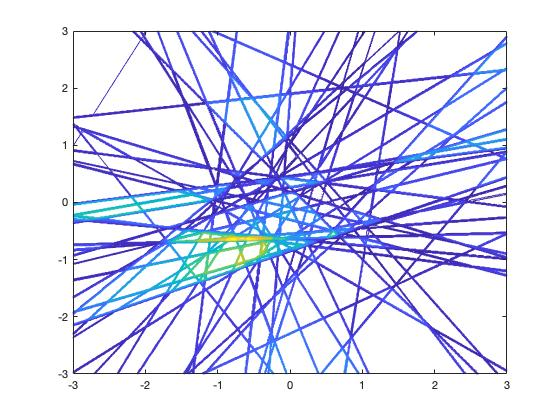
\includegraphics[width=.3\textwidth]{6dl/figures/dnn1-50.jpg}    
\end{center}
\caption{Hyperplanes with $\ell=1$, where $\ell$ is the depth of the neural network in \eqref{NNL}.}
\label{fig:1}
\end{figure} 		
 

The main goal of this section is to prove that the 
following type of error estimate holds, for some $\delta\ge 0$,
\begin{equation}\label{VNerror}
\inf_{v_N\in V_N^k}\|u- v_N \|_{H^m(\Omega)} \lesssim 
N^{-{1\over 2}-\delta}.
\end{equation} 
We will use two different approaches to establish \eqref{VNerror}.
The first approach, presented in \S\ref{sec:Bsplines}, mainly follows
\cite{hornik1994degree} and \cite{siegel2020approximations} that gives
error estimates for a general class of activation functions.  The
second approach follows
\cite{klusowski2016uniform} that gives error estimates specifically
for ReLU activation function.

We assume that $\Omega\subset\mathbb R^d$ is a given bounded domain.
Thus,
\begin{equation}
  \label{T}
T=\max_{x\in \bar{\Omega}} \|x\|<\infty.  
\end{equation}
The activation function ${\rm [ ReLU]}^k$ \eqref{relup} is related to
cardinal B-Splines.  A cardinal B-Spline of degree $k\ge 0$
denoted by $b^k$, is defined by convolution as
\begin{equation}
	b^k(x)=(b^{k-1}*b^0)(x)=\int_\mathbb{R}b^{k-1}(x-t)b^0(t)dt,
\end{equation}
where 
\begin{equation}
b^0(x)=\left\{
		     \begin{array}{lr}
		    1 & x\in[0,1),\\
		    0 & \hbox{otherwise}.
		     \end{array}
	\right.
\end{equation}
\begin{figure}
\begin{center}
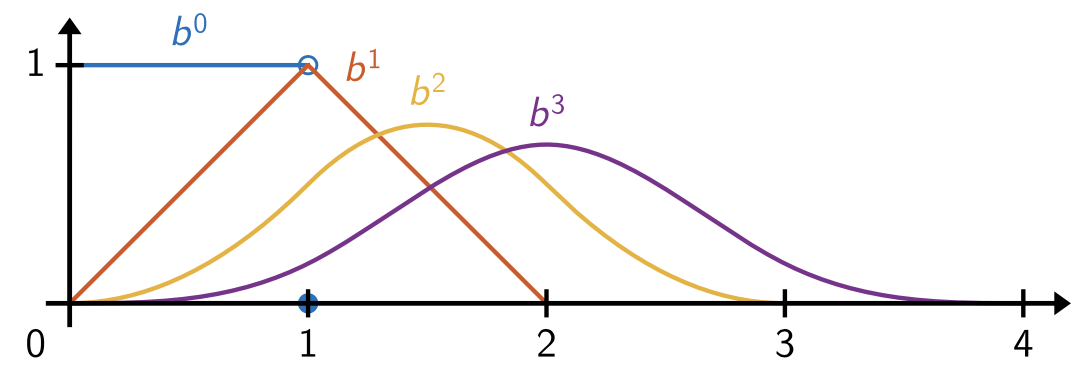
\includegraphics[width=0.5\textwidth]{6DL/figures/B-spline.png}   
\caption{Plots of some B-spline basis}
\label{bk}
\end{center}
\end{figure}
More explicitly, see \cite{de1971subroutine}, for any
$x\in[0,k+1]$ and $k\geq 1$, we have 
	\begin{equation}
	b^k(x)=\frac{x}{k}b^{k-1}(x)+\frac{k+1-x}{k}b^{k-1}(x-1),
	\end{equation}
or
	\begin{equation}\label{splinetorelu}
	b^k(x)=(k+1)\sum_{i=0}^{k+1} w_i(i-x)_+^k \hbox{~and~} w_i={\displaystyle\prod_{j=0,j\neq i}^{k+1}} \frac{1}{i-j}.
	\end{equation}
We note that all $b^k$ are locally supported and see Fig.~\ref{bk} for their plots. 

For an uniform grid with mesh size $h=\frac{1}{n+1}$, we define
	\begin{equation}
	b^k_{j,h}(x)=b^{k}(\frac{x}{h}-j).
	\end{equation}
Then the cardinal B-Spline series of degree $k$ on the uniform grid is 
\begin{equation}\label{Skn}
S_N^k=\Big\{v(x)=\sum_{j=-k}^{N}	c_jb^k_{j,h}(x)\Big\}.
\end{equation}
\begin{lemma} For $V_N^k$ and $S_N^k$ defined by \eqref{VkN} and
  \eqref{Skn}, we have
\begin{equation}
    \label{SV}
S_N^k\subset V_{N+k+1}^k.    
  \end{equation}
As a result, for any bounded domain $\Omega\subset \mathbb R^1$, we have
\begin{equation}
  \label{SVerror}
\inf_{v\in V_{N}^k}\|u-v\|_{m,\Omega} 
\le \inf_{v\in S_{N-k-1}^k}\|u-v\|_{m,\Omega} \lesssim N^{m-(k+1)} \|u\|_{k+1,\Omega}.
\end{equation}
\end{lemma}

\iffalse
Given an activation function $\sigma\in L^1(\mathbb R)$, consider its Fourier transformation:
\begin{equation}
  \label{Fsigma}
\hat \sigma(a) = \frac{1}{2\pi}\int_{\mathbb{R}} \sigma(t)e^{-iat}dt. 
\end{equation}
For any $a\neq 0$ with $\hat \sigma(a)\neq 0$, by making a change of variables 
$t = a^{-1}\omega\cdot x + b$ and $dt = db$, we have
 \begin{equation}
 \begin{aligned}
\hat{\sigma}(a)&=\frac{1}{2\pi}\int_{\mathbb{R}}\sigma(a^{-1}\omega\cdot x+b)e^{-ia( a^{-1}\omega\cdot x+b)}db = e^{-i\omega \cdot x}\frac{1}{2\pi}\int_{\mathbb{R}}\sigma(a^{-1} \omega\cdot x+b)e^{-iab}db.
 \end{aligned}
 \end{equation}
This implies that
\begin{equation}\label{FourierExp}
 e^{i\omega \cdot x} = \frac{1}{2\pi\hat{\sigma}(a)}\int_{\mathbb{R}}\sigma(a^{-1}\omega\cdot x+b)e^{-iab}db.
\end{equation}
We write $ \hat{u}(\omega) = e^{-i\theta(\omega)} | \hat{u}(\omega)|$
and then obtain the following integral represntation:
\begin{equation}\label{integral_representation01}
u(x) = \int_{\mathbb{R}^d} e^{i\omega\cdot x}\hat{u}(\omega)d\omega = 
\int_{\mathbb{R}^d}\int_\mathbb{R}\frac{1}{2\pi\hat{\sigma}(a)}
\sigma\left(a^{-1} \omega\cdot x+b\right)|\hat{u}(\omega)|e^{-i(ab+\theta(\omega))}dbd\omega
\end{equation}
Now we consider activation function $\sigma(x)=b^k(x)$ and $\hat \sigma$ be the
Fourier transform of $\sigma(x)$. Note that, by \eqref{bk}, 
\begin{align}\label{splineFourier}
\hat{\sigma}(a)=\left({1-e^{-ia}\over ia}\right)^{k+1}=\left({2\over a}\sin {a\over 2}\right)^{k+1}e^{-{ia(k+1)\over 2}}.
\end{align}

We first take $a=\pi$ in \eqref{splineFourier}. Thus,
\begin{equation}
  \label{pi1}
\hat\sigma(\pi)=
\left({2\over \pi}\right)^{k+1}e^{-{i\pi (k+1)\over 2}}.
\end{equation}
Combining \eqref{integral_representation01} and \eqref{pi1}, we obtain
that
\begin{equation}
  \label{splinerep0}
u(x) = 
\frac{1}{4}\left({\pi\over 2}\right)^{k}\int_{\mathbb{R}^d}\int_\mathbb{R}
\sigma\left(\pi^{-1}\omega\cdot x+b\right)|\hat{u}(\omega)|e^{-i(\pi b + {\pi (k+1)\over 2}+\theta(\omega))}dbd\omega
\end{equation}
An application of the Monte Carlo method in Lemma \ref{MC} to the integral representation \eqref{splinerep0} leads to the following estimate.
\begin{theorem}\label{splinestratify}
For any $0\le m\le k$, if $u\in {B}^{m+1}(\Omega)$, there exist $\omega_i\in \mathbb{R}^d$, $b_i\in \mathbb{R}$ such that
\begin{equation}
\left \|u - u_{N}\right\|_{H^{m}(\Omega)}\lesssim  N^{-{1\over 2}} \|u\|_{{B}^{m+1}(\Omega)}
\end{equation}
with
\begin{equation}
u_{N}(x)=\sum_{i=1}^{N} \beta_i b^k\left(\pi^{-1} \omega_i\cdot x+b_i\right).
\end{equation} 
\end{theorem}

Based on the integral representation \eqref{splinerep0}, a stratified analysis similar to the one in \cite{siegel2020approximations} leads to the following result.
\begin{theorem}
For any $0\le m\le k$ and positive $\epsilon$,  if $u\in {B}^{m+1+\epsilon}(\Omega)$, , there exist $\omega_i\in \mathbb{R}^d$, $b_i\in \mathbb{R}$ such that
\begin{equation}\label{straunbdd}
\left\|u - u_{N}\right\|_{H^{m}(\Omega)}\le  N^{-{1\over 2}-{\epsilon \over (d+1)(2+\epsilon)}} \|u\|_{{B}^{m+1+\epsilon}(\Omega)}
\end{equation}
with
\begin{equation}
u_{N}(x)=\sum_{i=1}^{N} \beta_i b^k\left(\bar \omega_i\cdot x+b_i\right) .
\end{equation} 
\end{theorem}
Next, we try to improve the estimate \eqref{straunbdd}. Again, we will use \eqref{integral_representation01}. Let $\displaystyle a_\omega=4\pi\lceil {\|\omega\|\over 4\pi}\rceil + \pi$ in \eqref{splineFourier} and $\displaystyle \bar\omega ={\omega\over a_\omega}$. We have
 \begin{equation}
\hat{\sigma}(a_\omega)=\left({2\over a_\omega}\right)^{k+1}, \quad \|\omega\| + \pi\le a_\omega\le \|\omega\|+5\pi,\quad \|\bar\omega\|\le 1,
 \end{equation}
which, together with \eqref{integral_representation01}, indicates that
 \begin{equation}\label{integral_representation}
 \begin{split}
  u(x) =  \int_{\mathbb{R}^d}\int_\mathbb{R}\frac{1}{2\pi}
  \sigma\left(\bar \omega\cdot x+b\right)\left({a_\omega\over 2}\right)^{k+1}\hat{u}(\omega)e^{-ia_\omega(b+{k+1\over 2})}dbd\omega.
\end{split}
 \end{equation}


\begin{theorem}
If $u\in {B}^{k+1}(\Omega)$, there exist $\|\bar \omega_i\|\le 1$, $|b_i|\le T + k+1$ such that
\begin{equation}\label{d+1}
\left\|u - u_{N}\right\|_{H^{m}(\Omega)}\lesssim  N^{-{1\over 2}-{1\over d+1}} \|u\|_{{B}^{k+1}(\Omega)}
\end{equation}
with
\begin{equation}
u_{N}(x)=\sum_{i=1}^{N} \beta_i b^k\left(\bar \omega_i\cdot x+b_i\right) .
\end{equation} 
\end{theorem}
\begin{proof}
We write \eqref{integral_representation} as follows
$$
\displaystyle u(x)= \int_{\mathbb{R}^d}\int_\mathbb{R}
g(x, b, \omega)\rho(b,\omega) dbd\omega
$$
with 
$$ 
\hat{u}(\omega) = e^{-i\theta(\omega)} | \hat{u}(\omega)|,\quad \tilde \theta(\omega)=\theta(\omega) + a_\omega(b+{k+1\over 2})
$$ and 
\begin{equation}\label{eq:g}
g(x, b, \omega) = \sigma\left({\bar \omega}\cdot x+b\right)sgn(\cos \tilde\theta(\omega)),
\end{equation}
\begin{equation}\label{eq:rho}
\rho(b,\omega) = \frac{1}{(2\pi)^d}\left({a_\omega\over 2}\right)^{k+1}| \hat{u}(\omega)||\cos \tilde\theta(\omega)|.
\end{equation} 
Note that
\begin{equation}
\|\bar\omega\|\le 1, \quad |b|\le T+k+1.
\end{equation} 
Let 
$$
G=\{(\omega, b): \omega\in \mathbb{R}^d,\ |b|\le T+k+1\}, \ \tilde G=\{(\bar \omega, b): \|\bar \omega\| \le 1,\ |b|\le T+k+1\}.
$$
For any positive integer $n$, divide $\tilde  G$ into $\tilde  M(\tilde  M\le {n\over 2})$   nonoverlapping subdomains, say 
$\tilde  G=\tilde  G_1\cup \tilde  G_2\cup \cdots \cup\tilde  G_{\tilde M}$, such that
\begin{equation}
|b-b'|\lesssim n^{-{1\over d+1}},\quad |\bar\omega - \bar\omega'|\lesssim  n^{-{1\over d+1}}, \quad (\bar\omega, b),\ (\bar\omega', b')\in \tilde G_i,\ 1\le i\le \tilde M.
\end{equation} 
Define $M=2\tilde  M$ and for $1\le i\le \tilde M$,
$$
G_i = \{(\omega, b): (\bar \omega, b)\in \tilde  G_i, \ \cos \tilde\theta(\omega)\ge 0\},\ 
G_{\tilde  M+i} = \{(\omega, b): (\bar \omega, b)\in \tilde  G_i, \ \cos \tilde\theta(\omega)\le 0\}.
$$
Thus, $G=G_1\cup G_2\cup \cdots \cup G_M$ with $\tilde  G_i\cap \tilde G_j=\varnothing$ if $i\neq j$, and 
\begin{equation}
|b-b'|\lesssim n^{-{1\over d+1}},\quad |\bar\omega - \bar\omega'|\lesssim  n^{-{1\over d+1}}, \quad sgn(\cos \tilde\theta(\omega))=sgn(\cos\tilde \theta(\omega')).
\end{equation} 
Let $n_i=\lceil \lambda(G_i)n\rceil$, $N=\displaystyle \sum_{i=1}^M n_i$ and
\begin{equation}
u_{N}(x)=\|\rho\|_{L^1(G)}\sum_{i=1}^{M} \frac{\lambda(G_{i})}{n_{i}} \sum_{j=1}^{n_{i}}g(x,\theta_{i,j}).
\end{equation}
It holds that
\begin{equation}\label{eq:sum}
\begin{split}
\mathbb{E}\left(\left\|u - u_{N}\right\|_{H^{m}(\Omega)}^{2}\right)\le&
\|\rho\|_{L^1(G)}\sum_{i=1}^{M}  \frac{\lambda^2(G_i)}{n_{i}}  \sup_{\theta_{i},\theta_{i}'\in G_i} \| g(x,\theta_i) - g(x,\theta_i')\|^2_{H^m(\Omega)}
 \end{split}
\end{equation}
with $\theta=(b, \omega)$. 
For any $(b, \omega)\in G_i$, $1\le i\le M$, if $k\ge m+1$,
\begin{equation}
|g(x,\theta) - g(x,\theta')| \lesssim |b-b'| + |\omega - \omega'| \lesssim   n^{-{1\over d+1}}
\end{equation}
Thus,
\begin{equation}
 \sum_{i=1}^{M}  \frac{\lambda^2(G_i)}{n_{i}}  \sup_{\theta_{i},\theta_{i}'\in G_i} \| g(x,\theta_i) - g(x,\theta_i')\|^2_{H^m(\Omega)}  
 \lesssim  n^{-{2\over d+1}} |\Omega|.
\end{equation}
Thus,
\begin{equation}\label{eq:}
\begin{split}
\mathbb{E}\left(\left\|u - u_{N}\right\|_{H^{m}(\Omega)}^{2}\right)\lesssim&   n^{-1-{2\over d+1}} |\Omega|\|\rho\|_{L^1(G)}.
 \end{split}
\end{equation}
Since $a\le \|\omega\|+5\pi$, 
$$
\|\rho\|_{L^1(G)}\lesssim \int_G (\|\omega\| + 1)^{k+1}|\hat u(\omega)|d\omega db \lesssim \|u\|_{B^{k+1}(\Omega)}.
$$
Note that $n\le N\le 2n$. Thus, there exist $\omega_i\in \mathbb{R}^d$, $\beta_i$, $b_i\in \mathbb{R}$ such that
\begin{equation}
\left\|u - u_{N}\right\|_{H^{m}(\Omega)}\lesssim  N^{-{1\over 2}-{1\over d+1}} \|u\|_{B^{k+1}(\Omega)},
\end{equation}
which completes the proof.
\end{proof}

The above analysis can also be applied to more general activation functions with compact support. 
\begin{theorem}
Suppose that $\sigma\in W^{m+1,\infty}(\mathbb{R})$ that has a compact
support. If for any $a>0$, there exists $\tilde a>0$ such that
\begin{equation}
\tilde a\gtrsim a,\quad  |\hat\sigma(\tilde a)|\gtrsim a^{-\ell},
\end{equation}
and  $u\in {B}^{\ell}(\Omega)$, then, there exist $\omega_i\in \mathbb{R}^d$ and $b_i\in \mathbb{R}$ such that
\begin{equation}
\left\|u - u_{N}\right\|_{H^{m}(\Omega)}\lesssim  N^{-{1\over 2}-{1\over d+1}} \|u\|_{B^{\ell}(\Omega)},
\end{equation}
where
\begin{equation}
u_{N}(x)=\sum_{i=1}^{N} \beta_i \sigma\left(\bar \omega_i\cdot x+b_i\right) .
\end{equation} 
\end{theorem}

\fi

%\subsection{ReLU Fourier representation }%-- Simple version}

We introduce the Taylor expansion of $e^{iz}$ with integral remainder as follows.
\begin{lemma}
For $|z|\leq c$, 
\begin{equation}  
e^{iz} -  iz -1
= 
- \int_{0}^c\left[(z - u)_+e^{iu} + (-z - u)_+e^{-iu} \right]du.
\end{equation}  
\end{lemma}
\begin{proof}  
By the Taylor expansion with integral remainder,
\begin{equation} 
e^{iz} = 1 + iz  - \int_0^z e^{iu}(z-u)du.
\end{equation}
Let $u_+=\max (u, 0)$ and $u_-=\min(u,0)$. Then, $u_-=-(-u)_+$ and 
$$
z-u=(z-u)_+ + (z-u)_-=(z-u)_+ - (u-z)_+.
$$
It follows that
\begin{equation}
\begin{split}
\int_{0}^z (z-u)e^{iu} du=&\int_{0}^z (z-u)_+e^{iu} du + \int_{0}^z -(u-z)_+e^{iu} du
\\
=&\int_{0}^z (z-u)_+e^{iu} du + \int_{0}^{-z}  (-u-z)_+e^{-iu} du
\\
=&\int_{0}^c (z-u)_+e^{iu} du + (-u-z)_+e^{-iu} du.
\end{split}
\end{equation}
Thus,
\begin{equation}  
e^{iz} - 1 - iz 
= 
-\int_{0}^c\left[(z - u)_+e^{iu} + (-z - u)_+e^{-iu} \right]du,
\end{equation}  
which completes the proof.
\end{proof}

Let $z=\omega\cdot x$, $u=\|\omega\|_{\ell_1}t$ and $\bar \omega={\omega\over \|\omega\|_{\ell_1}}$. If $\Omega$ is bounded, say $|x|\le T$, $|\bar \omega \cdot x|\le T$. There exists the following expansion for $e^{i\omega\cdot x}$.
\begin{lemma}\label{lm:talorcomplex}
If $|x|\le T$,
\begin{equation}  
e^{i\omega\cdot x} - 1 -  i\omega\cdot x 
= 
- \|\omega\|_{\ell_1}^2\int_{0}^T\left[(\bar \omega\cdot x - t)_+e^{i\|\omega\|_{\ell_1}t}
+ (-\bar \omega\cdot x - t)_+e^{-i\|\omega\|_{\ell_1}t} \right]dt.
\end{equation} 
Denote 
$$
D^\alpha = \partial_1^{\alpha_1}\partial_2^{\alpha_2}\cdots \partial_d^{\alpha_d},\quad \omega^\alpha = \omega_1^{\alpha_1}\omega_2^{\alpha_2}\cdots \omega_d^{\alpha_d},\quad \alpha!=\alpha_1!\alpha_2!\cdots \alpha_d!.
$$
\end{lemma}
It follows  the following Taylor expansion with an integral remainder.
\begin{lemma}\label{lm:probabilityexpan}
Suppose $|x|\le T$. There exists
\begin{equation}
f(x) = f(0) + \nabla f(0)\cdot x
+  \int_{\{-1,1\}\times [0,T]\times \mathbb{R}^{d}}  g(x, \theta)\lambda(\theta)d\theta  
\end{equation}  
with  $g(x,\theta)$ and $\lambda(\theta)$ defined in \eqref{eq:straglam}.
\end{lemma}
\begin{proof}
Since $
 f(x) = \int_{\mathbb{R}^d} e^{i\omega\cdot x}\hat{f}(\omega)d\omega
$
and 
$
\nabla f(x)=\int_{\mathbb{R}^d} i^{|\alpha|}\omega  e^{i\omega\cdot x}\hat{f}(\omega)d\omega,
$
\begin{eqnarray}
\nabla  f(0)\cdot x=\int_{\mathbb{R}^d} i\omega\cdot  x\hat{f}(\omega)d\omega.
\end{eqnarray} 
 It follows that
\begin{equation}
\nabla  f(0) \cdot x=i \int_{\mathbb{R}^d} \omega\cdot x\hat{f}(\omega)d\omega
=  \int_{\mathbb{R}^d} i\omega\cdot x\hat{f}(\omega)d\omega.
\end{equation} 
Let $\hat{f}(\omega)=|\hat{f}(\omega)|e^{ib(\omega)}$. Then, $e^{i\|\omega\|_{\ell_1}t}\hat{f}(\omega) = |\hat{f}(\omega)|e^{i(\|\omega\|_{\ell_1}t + b(\omega))}$.
By Lemma \ref{lm:talorcomplex},
\begin{equation}\label{eq:fftaylor}
\begin{split}
&f(x) - f(0) - \nabla  f(0) \cdot x
\\
= &\int_{\mathbb{R}^d} \big (e^{i\omega\cdot x} - 1 - i\omega\cdot x \big )\hat{f}(\omega)d\omega.
\\
=&{\rm Re} \bigg (-\int_{\mathbb{R}^d} \int_{0}^T\left[(\bar \omega\cdot x - t)_+e^{i\|\omega\|_{\ell_1}t}
+ (-\bar \omega\cdot x - t)_+e^{-i\|\omega\|_{\ell_1}t} \right]\hat{f}(\omega)\|\omega\|_{\ell_1}^{2}dt d\omega\bigg )
\\
=& \int_{\{-1,1\}}\int_{\mathbb{R}^d} \int_{0}^T (z\bar \omega\cdot x - t)_+ s(zt,\omega)  |\hat{f}(\omega)|\|\omega\|_{\ell_1}^{2}dtd\omega dz
\end{split}
\end{equation}
with $\int_{\{-1, 1\}} r(z) dz = r(-1) + r(1)$ and
\begin{equation} 
s(zt,\omega)= -\cos(z\|\omega\|_{\ell_1}t + b(\omega)) 
\end{equation} 
Define $G=\{-1,1\}\times [0,T]\times \mathbb{R}^{d}$, $\theta=(z, t, \omega)\in G$,
\begin{equation}\label{eq:straglam}
g(x,\theta)= (z\bar \omega\cdot x - t)_+ {\rm sgn} s(zt,\omega),\qquad \lambda(\theta)={\rho(\theta)\over 
\int_{\{-1,1\}\times [0,T]\times \mathbb{R}^{d}} \rho(\theta)d\theta}.
\end{equation}
with $\rho(\theta) = |s(zt,\omega)||\hat{f}(\omega)|\|\omega\|_{\ell_1}^{2}$. 

Then \eqref{eq:fftaylor} can be written as 
\begin{equation}\label{eq:reluintegral}
f(x) = f(0) +  \nabla  f(0) \cdot x
+  \int_{\{-1,1\}\times [0,T]\times \mathbb{R}^{d}}  g(x, \theta)\lambda(\theta)d\theta,  
\end{equation}   
which completes the proof.
\end{proof}

An application of the Monte Carlo method in Lemma \ref{MC} to the integral \eqref{eq:reluintegral} gives the following estimate.
\begin{theorem} 
Suppose $|x|\le T$ and 
$$
 \int_{\mathbb{R}^{d}} |\hat{f}(\omega)|\|\omega\|_{\ell_1}^{2} d\omega<\infty.
$$
There exist  $\|\bar \omega_j\|_{\ell_1}=1$, $t\in [0,T]$ such that 
$$
f_n(x)= f(0) + \nabla  f(0) \cdot x  + {1\over n}\sum_{j=1}^{n} (\bar \omega_j\cdot x - t_j)_+
$$ 
satisfies the following estimate 
\begin{equation}
\|f - f_n \|_{L^2(\Omega)} \leq C n^{-{1\over 2}}.
\end{equation} 
%\begin{equation}
%\|D^\beta (f(x)- f_n(x))\|_{L^2(\Omega)}\le \sqrt{2^{m-k-2}(2m-k)\over k!(m-k)!}|\Omega|^{1/2} n^{-{1\over 2}-{1\over d}},\quad |\beta|=k\le m.
%\end{equation}
\end{theorem}

\iffalse
\noindent\textbf{A modified analysis using stratified sampling}

According to \eqref{eq:straglam}, the main ingredient $(z\bar \omega\cdot x - t)_+$ of $g(x,\theta)$  only includes the direction $\bar\omega$ of $\omega$ which belongs to a bounded domain  $\mathbb{S}^{d-1}$. Thanks to the continuity of $(z\bar \omega\cdot x - t)_+$ with respect to $(z, \bar\omega, t)$ and the boundedness of $\mathbb{S}^{d-1}$,
the application of the stratified sampling to the residual term of the Taylor expansion leads to the following approximation property.
\begin{theorem}\label{est:stratify}
Suppose $|x|\le T$ and 
$$
 \int_{\mathbb{R}^{d}} |\hat{f}(\omega)|\|\omega\|_{\ell_1}^{2} d\omega<\infty.
$$
There exist $\beta_j\in [-2^d,2^d]$, $\|\bar \omega_j\|_{\ell_1}=1$, $t\in [0,T]$ such that 
$$
f_n(x)= f(0) + \nabla  f(0) \cdot x  + {1\over n}\sum_{j=1}^{n}\beta_j (\bar \omega_j\cdot x - t_j)_+
$$ 
satisfies the following estimate 
\begin{equation}
\|f - f_n \|_{L^2(\Omega)} \leq C n^{-{1\over 2}-{1\over d}}.
\end{equation} 
%\begin{equation}
%\|D^\beta (f(x)- f_n(x))\|_{L^2(\Omega)}\le \sqrt{2^{m-k-2}(2m-k)\over k!(m-k)!}|\Omega|^{1/2} n^{-{1\over 2}-{1\over d}},\quad |\beta|=k\le m.
%\end{equation}
\end{theorem}
\begin{proof}
By Lemma \ref{lem:stratifiedapprox}, for any decomposition $G=\cup_{i=1}^M G_i$, there exist $\{\theta_i\}_{i=1}^n$ and $\{\beta_i\}_{i=1}^n\in [0,1]$ such that 
\begin{equation}
\|  f - f_n\|_{L^2(\Omega)} = \|  r - r_{n}\|_{L^2(\Omega)} \leq {1\over n^{1/2}}\max_{1\le j\le M}\sup_{\theta_{j},\theta_{j}'\in G_j} \|   g(x,\theta_j) - g(x,\theta_j') \|_{L^2(\Omega)} 
\end{equation}
with 
$$
f_n(x)= f(0) +  \nabla  f(0) \cdot x + r_{n}(x), \qquad r_{n}(x)={1\over n}\sum_{j=1}^{n}\beta_j (\bar \omega_j\cdot x - t_j)_+, 
$$
$$
r(x)=\int_{\{-1,1\}\times [0,T]\times \mathbb{R}^{d}}  g(x, \theta)\lambda(\theta)d\theta.
$$
Consider a particular decomposition $G=\cup_{i=1}^M G_i$ as follows. 
The variable $z$ is in the set $\{-1,1\}$, which can be divided into two subsets $\{-1\}$ and $\{1\}$. 
Given a positive integer $n$, for the random variable $t$, the interval  $ [0,T]$ can be divided into $n_t$ subintervals $\{G_i^t\}_{i=1}^{n_t}$ such that 
$$
|t-t'|<{1\over 2}n^{-{1\over d}}\quad t,t'\in G_i^t,\quad 1\leq i\leq n_t
$$ 
for $n_t>2\lceil T  n^{1\over d}\rceil$. 
For variable $\bar \omega=\omega/\|\omega\|_{\ell_1}\in \mathbb{S}^{d-1}$ where $\mathbb{S}^{d-1}=\{\bar \omega\in \mathbb{R}^d: \|\bar \omega\|_{\ell_1}=1\}$. Note that $\mathbb{S}^{d-1}$ can be divided into $n_\alpha$ subdomains $\{G_i^s \}_{i=1}^{n_s}$ such that
$$
\|\bar \omega- \bar \omega'\|_{\ell_1}\leq {1\over 2}n^{-{1\over d}}\qquad \bar \omega, \bar \omega' \in G_i^s,\quad 1\leq i\leq n_s
$$
for $(2n^{1\over d})^{d-1}\leq n_s\leq \lceil (5n^{1\over d})^{d-1}\rceil$ \cite{klusowski2016uniform}.
Then 
$$
G=\displaystyle \cup \{G_{ijk\ell}: 1\leq i\leq 2,\ 1\leq j\leq n_t,\ 1\leq k\leq n_s,\ 1\le \ell\le 2\}
$$
with 
\begin{equation}
G_{ijk\ell} = \{(z, t, \omega): z=(-1)^i,\ t\in G_j^t, \bar \omega \in G_k^s,\ {\rm sgn} s(zt,\omega)=(-1)^\ell\}.
\end{equation}
Denote this decomposition of $G$ by $G=\cup_{i=1}^{M} G_i$ with $M=4n_sn_t\le 2^{d}n$. For each $G_i$,
\begin{equation}
z=z',\ |t-t'|<{1\over 2}n^{-{1\over d}},\ \|\bar \omega  - \bar \omega'\|_{\ell^1}<{1\over 2}n^{-{1\over d}}\qquad \forall \theta=(z, t, \omega),\ \theta'=(z', t', \omega')\in G_i.
\end{equation}
For any $\theta_i, \theta'_i\in G_i$ and $|\alpha |=1$,  
$$
| g(x,\theta_i) - g(x,\theta_i') | =  | \bar\omega  -   \bar\omega' |\le n^{-{1\over d}}.
$$  
Thus, there exist $\theta_{i,j}$ such that
\begin{equation}
\| f - f_n\|_{L^2(\Omega)} \le C  n^{-{1\over 2}-{1\over d}}.
\end{equation}
with
$$
f_n(x)=  f(0) + \nabla f(0) \cdot x + {1\over  n}\sum_{j=1}^{n}\beta_j (\bar \omega_j\cdot x - t_j)_+
$$ 
with $\beta_j\in [-2^d,2^d]$,
which completes the proof.
\end{proof}


\fi
 

















%\section{ReLU Fourier representation}\label{sec:error2}
Rather than using general Fourier transform  to represent
$e^{i\omega\cdot x}$ in terms of $\sigma(\omega\cdot x+b)$, 
\cite{klusowski2016uniform} gave a different method to represent
$e^{i\omega\cdot x}$ in terms of $(\omega\cdot x+b)_+^k$  for $k=1$
and $2$.   The following lemma gives a generalization of this
representation for all $k\ge 0$. 
\begin{lemma}\label{lm:talorcomplex}
For any $k\ge0$ and $x\in \Omega$,
\begin{equation}  
e^{i\omega\cdot x} =\sum_{j=0}^k{(i\omega\cdot x)^{j}\over j!} 
+
{i^{k+1}\over k!} \|\omega\|^{k+1}\int_{0}^T\left[(\bar \omega\cdot x - t)_+^ke^{i\|\omega\|t}
+(-1)^{k-1}(-\bar \omega\cdot x - t)_+^ke^{-i\|\omega\|t} \right]dt.
\end{equation} 
\end{lemma}
\begin{proof}  
For $|z|\leq c$, by the Taylor expansion with integral remainder,
\begin{equation} 
e^{iz} = \sum_{j=0}^k {(iz)^j\over j!} + {i^{k+1}\over k!} \int_0^z e^{iu}(z-u)^kdu.
\end{equation}
Note that 
$$
(z-u)^k=(z-u)^k_+ - (u-z)^k_+.
$$
It follows that
\begin{equation}
\begin{split}
\int_{0}^z (z-u)^ke^{iu} du=&\int_{0}^z (z-u)_+^ke^{iu} du + \int_{0}^z (-1)^k(u-z)_+^ke^{iu} du
\\
=&\int_{0}^z (z-u)_+^ke^{iu} du + \int_{0}^{-z} (-1)^{k-1}(-u-z)_+^ke^{-iu} du
\\
=&\int_{0}^c (z-u)_+^ke^{iu} du + (-1)^{k-1}(-u-z)_+^ke^{-iu} du.
\end{split}
\end{equation}
Thus,
\begin{equation}  
e^{iz} - \sum_{j=0}^k{(iz)^{j}\over j!} 
= 
{i^{k+1}\over k!}\int_{0}^c\left[(z - u)_+^ke^{iu} + (-1)^{k-1}(-z - u)_+^ke^{-iu} \right]du.
\end{equation}  
Let 
\begin{equation}\label{baromega}
z=\omega\cdot x,\quad u=\|\omega\|t,\quad \bar \omega={\omega\over \|\omega\|}.
\end{equation}
Since $\|x\| \le T$ and $|\bar \omega \cdot x|\le T$, we obtain
\begin{equation}  
e^{i\omega\cdot x} - \sum_{j=0}^k{(i\omega\cdot x)^{j}\over j!} 
= 
{i^{k+1}\over k!} \|\omega\|^{k+1}\int_{0}^T\left[(\bar \omega\cdot x - t)_+^ke^{i\|\omega\|t}
+(-1)^{k-1}(-\bar \omega\cdot x - t)_+^ke^{-i\|\omega\|t} \right]dt,
\end{equation} 
which completes the proof.
\end{proof}

Since $
u(x) = {1\over (2\pi)^d}\int_{\mathbb{R}^d} e^{i\omega\cdot x}\hat{u}(\omega)d\omega
$
and 
$
 \partial^\alpha u(x)=\int_{\mathbb{R}^d} i^{|\alpha|}\omega^\alpha e^{i\omega\cdot x}\hat{u}(\omega)d\omega,
$
\begin{eqnarray}
 \partial^\alpha u(0)x^\alpha=\int_{\mathbb{R}^d} i^{|\alpha|}\omega^\alpha x^\alpha\hat{u}(\omega)d\omega.
\end{eqnarray} 
Note that $\displaystyle (\omega\cdot x)^j=\sum_{|\alpha|=j}{j!\over \alpha !}\omega^\alpha x^\alpha $. It follows that
\begin{equation}
\sum_{|\alpha|=j}{1\over \alpha!} \partial^\alpha u(0) x^\alpha=i^j\sum_{|\alpha|=j}{1\over \alpha!} \int_{\mathbb{R}^d} \omega^\alpha x^\alpha\hat{u}(\omega)d\omega
={1\over j!}  \int_{\mathbb{R}^d} (i\omega\cdot x)^j \hat{u}(\omega)d\omega.
\end{equation} 
Let $\hat{u}(\omega)=|\hat{u}(\omega)|e^{ib(\omega)}$. Then, $e^{i\|\omega\|t}\hat{u}(\omega) = |\hat{u}(\omega)|e^{i(\|\omega\|t + b(\omega))}$.
By Lemma \ref{lm:talorcomplex},
\begin{equation}\label{eq:fftaylor}
\begin{split}
&u(x) - \sum_{|\alpha|\le k}{1\over \alpha!} \partial^\alpha u(0) x^\alpha
\\
= &\int_{\mathbb{R}^d} \big (e^{i\omega\cdot x}-\sum_{j=0}^k{1\over j!}(i\omega\cdot x)^j\big )\hat{u}(\omega)d\omega.
\\
=&{\rm Re} \bigg ({i^{k+1}\over k!}\int_{\mathbb{R}^d} \int_{0}^T\left[(\bar \omega\cdot x - t)_+^ke^{i\|\omega\|t}
+(-1)^{k-1}(-\bar \omega\cdot x - t)_+^ke^{-i\|\omega\|_{\ell_1}t} \right]\hat{u}(\omega)\|\omega\|^{k+1}dt d\omega\bigg )
\\
=& {1\over k!}\int_{\{-1,1\}}\int_{\mathbb{R}^d} \int_{0}^T (z\bar \omega\cdot x - t)_+^k s(zt,\omega)  |\hat{u}(\omega)|\|\omega\|^{k+1}dtd\omega dz
\end{split}
\end{equation}
with $\int_{\{-1, 1\}} r(z) dz = r(-1) + r(1)$ and
\begin{equation} 
s(zt,\omega)= 
\begin{cases}
(-1)^{k+1\over 2}\cos(z\|\omega\|t + b(\omega)) & k \text{ is odd},
\\
(-1)^{k+2\over 2}\sin(z\|\omega\|t + b(\omega)) & k \text{ is even}.
\end{cases}
\end{equation} 
Define $G=\{-1,1\}\times [0,T]\times \mathbb{R}^{d}$, $\theta=(z, t, \omega)\in G$,
\begin{equation}\label{eq:straglam}
g(x,\theta)= (z\bar \omega\cdot x - t)_+^k {\rm sgn} s(zt,\omega),\qquad  \rho(\theta) = {1\over (2\pi)^d}|s(zt,\omega)||\hat{u}(\omega)|\|\omega\|^{k+1},\quad \lambda(\theta)={\rho(\theta)\over 
\|\rho\|_{L^1(G)}}.
\end{equation} 

Then \eqref{eq:fftaylor} can be written as 
\begin{equation}
u(x) = \sum_{|\alpha|\le k}{1\over \alpha!}D^\alpha u(0) x^\alpha
+ {\nu\over k!}\int_G  g(x, \theta)\lambda(\theta)d\theta,  
\end{equation}   
with $\nu=\int_G \rho(\theta)d\theta$. In summary, we have the following lemma.
 


\begin{lemma}\label{lm:probabilityexpan}
It holds that
\begin{equation}\label{ReLUm}
u(x) = \sum_{|\alpha|\le k}{1\over \alpha!} \partial^\alpha u(0) x^\alpha
+ {\nu\over k!}r_k(x),\qquad x\in \Omega
\end{equation}  
with $\nu=\int_G \rho(\theta)d\theta$ and 
\begin{equation}\label{ReLUrm}
r_k(x) = \int_G  g(x, \theta)\lambda(\theta)d\theta,\qquad G=\{-1,1\}\times [0,T]\times \mathbb{R}^{d},
\end{equation}  
and  $g(x,\theta)$, $\rho(\theta)$  and $\lambda(\theta)$ defined in \eqref{eq:straglam}.
\end{lemma}

According to \eqref{eq:straglam}, the main ingredient $(z\bar
\omega\cdot x - t)_+^k$ of $g(x,\theta)$ only includes the direction
$\bar\omega$ of $\omega$ which belongs to a bounded domain
$\mathbb{S}^{d-1}$. Thanks to the continuity of $(z\bar \omega\cdot x
- t)_+^k$ with respect to $(z, \bar\omega, t)$ and the boundedness of
$\mathbb{S}^{d-1}$, the application of the stratified sampling to the
residual term of the Taylor expansion leads to the 
approximation property in Theorem \ref{est:stratify}.

\begin{theorem}\label{est:stratify}
Assume $u\in B^{k+1}(\Omega)$
%$$
% \int_{\mathbb{R}^{d}} |\hat{f}(\omega)|\|\omega\|^{m+1} d\omega<\infty.
%$$
There exist $\beta_j\in [-1, 1]$, $\|\bar \omega_j\|=1$, $t_j\in [0,T]$ such that 
\begin{equation}
u_N(x)= \sum_{|\alpha|\le k}{1\over \alpha!} \partial^\alpha u(0) x^\alpha + {2\nu\over k!N}\sum_{j=1}^{N}\beta_j (\bar \omega_j\cdot x - t_j)_+^k
\end{equation} 
with $\nu=\int_G \rho(\theta)d\theta$ and $\rho(\theta)$  defined in \eqref{eq:straglam} 
satisfies the following estimate
\begin{equation}
\|u - u_N \|_{H^m(\Omega)} \lesssim  
\begin{cases}
 N^{-{1\over 2}-{1\over d}}\|u\|_{B^{k+1}(\Omega)},&m< k,
\\
N^{-{1\over 2}}\|u\|_{B^{k+1}(\Omega)}& m=k.
\end{cases} 
\end{equation} 
%Especially,
%\begin{equation}
%\|u - u_N \|_{L^2(\Omega)} \leq {(2T)^k|\Omega|^{1\over 2}\over (k-1)!} N^{-{1\over 2}-{1\over d}}\|u\|_{\mathcal B^{k+1, q}(\Omega)}.
%\end{equation} 
%\begin{equation}
%\|D^\beta (f(x)- f_n(x))\|_{L^2(\Omega)}\le \sqrt{2^{m-k-2}(2m-k)\over k!(m-k)!}|\Omega|^{1/2} n^{-{1\over 2}-{1\over d}},\quad |\beta|=k\le m.
%\end{equation}
\end{theorem}

\begin{proof}
Let
$$
u_N(x)=  \sum_{|\alpha|\le k}{1\over \alpha!} \partial^\alpha u(0) x^\alpha + {\nu\over k!} r_{k,N}(x), \qquad r_{k,N}(x)={1\over N}\sum_{j=1}^{N}\beta_j (\bar \omega_j\cdot x - t_j)_+^k.
$$
Recall  the representation  of $u(x)$ in \eqref{ReLUm} and $r_k(x)$ in \eqref{ReLUrm}. It holds that
\begin{equation}
u(x) - u_N(x)={2\nu\over k!} (r_k(x) - r_{k,N}(x)).
\end{equation}
By Lemma \ref{lem:stratifiedapprox}, for any decomposition $\displaystyle G=\cup_{i=1}^N G_i$, there exist $\{\theta_i\}_{i=1}^N$ and $\{\beta_i\}_{i=1}^N\in [0, 1]$ such that 
\begin{equation}
\| \partial_x^\alpha (u - u_N)\|_{L^2(\Omega)} = {\nu\over k!}\|  \partial_x^\alpha (r_k - r_{k,N})\|_{L^2(\Omega)} \leq {1\over k!N^{1/2}}\max_{1\le j\le n}\sup_{\theta_{j},\theta_{j}'\in G_j} \|  \partial_x^\alpha \big(g(x,\theta_j) - g(x,\theta_j')\big)\|_{L^2(\Omega)}.
\end{equation}
\iffalse
Consider a $\epsilon$-covering decomposition $G=\cup_{i=1}^M G_i$ as follows. 
The variable $z$ is in the set $\{-1,1\}$, which can be divided into two subsets $\{-1\}$ and $\{1\}$. 
Given a positive integer $N$, for the random variable $t$, the interval  $ [0,T]$ can be divided into $n_t$ subintervals $\{G_i^t\}_{i=1}^{n_t}$ such that 
$$
|t-t'|<{1\over 2}N^{-{1\over d}}\quad t,t'\in G_i^t,\quad 1\leq i\leq n_t
$$ 
for $n_t>2\lceil T N^{1\over d}\rceil$. 
For variable $\bar \omega=\omega/\|\omega\|\in \mathbb{S}^{d-1}$ where $\mathbb{S}^{d-1}=\{\bar \omega\in \mathbb{R}^d: \|\bar \omega\|=1\}$. Note that $\mathbb{S}^{d-1}$ can be divided into $n_\alpha$ subdomains $\{G_i^s \}_{i=1}^{n_s}$ such that
$$
\|\bar \omega- \bar \omega'\|\leq {1\over 2}N^{-{1\over d}}\qquad \bar \omega, \bar \omega' \in G_i^s,\quad 1\leq i\leq n_s
$$
for $(2N^{1\over d})^{d-1}\leq n_s\leq \lceil (5N^{1\over d})^{d-1}\rceil$ \cite{klusowski2016uniform}.
Then 
$$
G=\displaystyle \cup \{G_{ijk\ell}: 1\leq i\leq 2,\ 1\leq j\leq n_t,\ 1\leq k\leq n_s,\ 1\le \ell\le 2\}
$$
with 
\begin{equation}
G_{ijk\ell} = \{(z, t, \omega): z=(-1)^i,\ t\in G_j^t, \bar \omega \in G_k^s,\ {\rm sgn} s(zt,\omega)=(-1)^\ell\}.
\end{equation}
Denote this decomposition of $G$ by $G=\cup_{i=1}^{M} G_i$ with $M=4n_sn_t\le 2^{d}N$. For each $G_i$,
\fi
Consider a $\epsilon$-covering decomposition $G=\cup_{i=1}^N G_i$  such that 
\begin{equation}
z=z',\ |t-t'|<\epsilon,\ \|\bar \omega  - \bar \omega'\|_{\ell^1}<\epsilon\qquad \forall \theta=(z, t, \omega),\ \theta'=(z', t', \omega')\in G_i
\end{equation}
where $\bar\omega$ is defined in \eqref{baromega}. 
For any $\theta_i, \theta'_i\in G_i$,  
$$
| \partial_x^\alpha \big (g(x,\theta_i) - g(x,\theta_i')\big )| = {k!\over (k-|\alpha|)!} | g_\alpha(x, \bar\omega, t) -  g_\alpha(x, \bar\omega', t')| 
$$
with 
\begin{equation}
 g_\alpha(x, \bar\omega, t)  = (z\bar \omega\cdot x-t)^{k-|\alpha|}_+\bar \omega^\alpha.
 \end{equation} 
 Since
$$
|\partial_{\bar\omega_i}  g_\alpha|\le (2T)^{m-|\alpha|-1}\big ((k-|\alpha|)x_i + 2T\alpha_i\big ), \qquad |\partial_t  g_\alpha|\le (k-|\alpha|)(2T)^{k-|\alpha|-1},
$$
it follows that
\begin{equation}
\big | \partial_x^\alpha \big (g(x,\theta_i) - g(x,\theta_i')\big )\big | \le {k!\over (k-|\alpha|)!}(2T)^{k-|\alpha|-1}   \bigg ( (k-|\alpha|)(|x|_{\ell_1}+1) + 2T|\alpha |\bigg ) \epsilon.
\end{equation}
Thus, by Lemma \ref{lem:stratifiedapprox}, if $m=|\alpha|<k$,
\begin{equation}
\|  \partial_x^\alpha (u - u_N)\|_{L^2(\Omega)} \le {|\Omega|^{1/2}\over (k-|\alpha|)!}(2T)^{k-|\alpha|-1}   \bigg ( (k-|\alpha|)(T+1) + 2T|\alpha |\bigg )N^{-{1\over 2}}\epsilon.
\end{equation}
Note that $\epsilon \sim N^{-{1\over d}}$. There exist $\theta_{i,j}$ such that for any $0\le k< m$,
\begin{equation}
\| u - u_N\|_{H^k(\Omega)} \le  C(m,k,\Omega)\nu N^{-{1\over 2}-{1\over d}}
\end{equation}
with $\nu\le \|u\|_{B^{k+1}(\Omega)}$ and
\begin{equation}\label{equ:defcmko}
C(m,k,\Omega)=|\Omega|^{1/2}\bigg (\sum_{|\alpha|\le k}{1\over (k-|\alpha|)!}(2T)^{k-|\alpha|-1}   \big ( (k-|\alpha|)(T+1) + 2T|\alpha |\big )\bigg )^{1/2}.
\end{equation} 
If $m=|\alpha|=k$,
$$
\max_{1\le j\le M}\sup_{\theta_{j},\theta_{j}'\in G_j} \| D_x^\alpha \big(g(x,\theta_j) - g(x,\theta_j')\big)\|_{L^2(\Omega)}\lesssim 1.
$$
This leads to 
\begin{equation}
\| u - u_N\|_{H^m(\Omega)} \le  C(m,k,\Omega)\nu N^{-{1\over 2}}\quad \mbox{for }\ k=m.
\end{equation}
Note that $u_N$ defined above can be written as
$$
u_N(x)=  \sum_{|\alpha|\le k}{1\over \alpha!} \partial^\alpha u(0) x^\alpha + {1\over k!N}\sum_{j=1}^{N}\beta_j (\bar \omega_j\cdot x - t_j)_+^k
$$ 
with $\beta_j\in [-1, 1]$,
which completes the proof.
\end{proof}

\begin{lemma}
There exist $\alpha_i$, $\omega_i$, $b_i$ and $N\le 2\begin{pmatrix} k+d\\k\end{pmatrix}$
such that
$$
 \sum_{|\alpha|\le m}{1\over \alpha!} \partial^\alpha u(0) x^\alpha = \sum_{i=1}^N\alpha_i (\omega_i\cdot x + b_i)_+^k
$$ 
with $
x^\alpha = x_1^{\alpha_1}x_2^{\alpha_2}\cdots x_d^{\alpha_d},\quad \alpha!=\alpha_1!\alpha_2!\cdots \alpha_d!.
$
\end{lemma}
The above result can be found in \cite{he2020preprint}

A combination of Theorem \ref{est:stratify} and the above the lemma gives the following estimate in Theorem \ref{th:stra}.
\begin{theorem} \label{th:stra}
Suppose $u\in B^{k+1}(\Omega)$.
There exist $\beta_j, t\in \mathbb{R}$, $\omega_j \in \mathbb{R}^d$ such that 
\begin{equation}
u_N(x)= \sum_{j=1}^{N}\beta_j (\bar \omega_j\cdot x - t_j)_+^k
\end{equation} 
satisfies the following estimate
\begin{equation}\label{d}
\|u- u_N \|_{H^m(\Omega)} \lesssim 
\begin{cases}
N^{-{1\over 2}-{1\over d}}\|u\|_{B^{k+1}(\Omega)},\qquad k> m,
\\
N^{-{1\over 2}}\|u\|_{B^{k+1}(\Omega)},\qquad k= m,
\end{cases}
\end{equation} 
where $\bar\omega$ is defined in \eqref{baromega}.
\end{theorem}

\begin{remark}
We make the following comparisons:
\begin{enumerate}
\item The results in \ref{sec:Bsplines} are for activation functions $\sigma=b_k$, while the results in Section \ref{sec:error2} are for activation functions $\sigma={\rm ReLU}^k$.
\item By \eqref{splinetorelu}, the following relation obviously holds
$$
V_N(b_k)\subset V_{N+k}({\rm ReLU}^k),
$$
where 
\begin{equation}
\label{VkN}
V_{N+k}({\rm ReLU}^k)=\left\{\sum_{i=1}^Na_i(w_i\cdot x+b_i)_+^k, a_i, b_i\in\mathbb R^1, w_i\in \mathbb R^{1\times d}\right\},
\end{equation}
and $V_N(b_k)$ is the one hidden layer neuron network
function class with activation function $b_k$.  Thus, asymptotically
speaking, the results that hold for $\sigma=b_k$ also hold for
$\sigma={\rm ReLU}^k$. 
\end{enumerate}
\end{remark}







\subsection{Periodic activation function}
By dilating $\sigma$ if necessary, we may assume without loss of generality that $\sigma$ is periodic on $[0,1]$. Consider the Fourier series of $\sigma$
\begin{equation}
\sigma(x) = \displaystyle\sum_{i=-\infty}^\infty a_i e^{2\pi ix},
\end{equation}
with coefficients
\begin{equation}\label{eq_1027}
a_i =  \int_0^{1} \sigma(b)e^{-2\pi ib}db. 
\end{equation}
The assumption that $\sigma$ is non-constant means that there exists some $i$ such that $a_i \neq 0$. Note that we do not need the Fourier series to converge pointwise to $\sigma$, all we need is for some $a_i$ to be non-zero and the integrals in \eqref{eq_1027} to converge (which is does since $\sigma\in W^{m,\infty}$). Notice that shifting $\sigma$ by $t$, i.e. replacing $\sigma$ by $\sigma(\cdot+t)$, scales the coefficient $a_i$ by $e^{it}$. Setting $t = (\omega \cdot x)$, we get
\begin{equation}
e^{2\pi i\omega\cdot x} = \frac{1}{a_i}\int_0^{1} \sigma\left(\omega\cdot x + b\right)e^{-2\pi ib}db.
\end{equation}
Plugging this into the Fourier representation of $u$, we see that
\begin{equation}
u(x) = \int_{\mathbb{R}^d} e^{2\pi i\omega\cdot x}\hat{u}(\omega)d\omega = \frac{1}{ a_i}
\int_{\mathbb{R}^d}\int_0^{1}\sigma\left(\omega\cdot x + b\right)e^{-2\pi ib}\hat{u}(\omega)dbd\omega.
\end{equation}
Since $u(x)$ is real, we can add this to its conjugate to obtain the representation
\begin{equation}\label{eq_1029}
u(x) = \int_{\mathbb{R}^d} e^{2\pi i\omega\cdot x}\hat{u}(\omega)d\omega = \frac{1}{|a_i|}
\int_{\mathbb{R}^d}\int_0^{1}\sigma\left(\omega\cdot x + b\right)e^{-ib}\hat{u}(\omega)dbd\omega.
\end{equation}
 
 

\endinput
 Since $f(x)$ is real-valued, it implies that, for $x, x_B\in B$
 \begin{equation}
 \label{key}
 \begin{aligned}
 f(x)-f(x_B)
 &={\rm Re}\int_{\mathbb{R}^d}
 (e^{i\omega\cdot x}-e^{i\omega\cdot x_B}) 
 \hat{f}(\omega)d\omega \\
 &={\rm Re}\int_{\mathbb{R}^d}
 (e^{i\omega\cdot x}-e^{i\omega\cdot x_B})  
 e^{i\beta
 	(\omega)}|\hat{f}(\omega)|d\omega \\
 &=\int_{\mathbb{R}^d}(\cos(\omega\cdot
 x+\beta(\omega))-\cos(\omega\cdot x_B+\beta(\omega)))|\hat{f}(\omega)|d\omega \\
 &=\int_{\mathbb{R}^d}(\cos(\omega\cdot(x-x_B)+\beta_B(\omega))-\cos(\beta_B(\omega)))|\hat{f}(\omega)|d\omega
 \end{aligned}
 \end{equation}
 where
 $$
 \beta_B(\omega)=\omega\cdot x_B+\beta(\omega),\quad|\omega|_B:=\sup\limits_{x\in B}|\omega\cdot(x-x_B)|
 $$
 \begin{lemma}
 	\begin{equation}
 	\label{eq:2}
 	f(x)-f(x_B)=\int_{\mathbb{R}^d}k(x,\omega)d\omega
 	\end{equation}
 	\begin{equation}
 	\label{eq:1}
 	k(x, \omega)=\cos(\omega\cdot(x-x_B)+\beta_B(\omega))-\cos(\beta_B(\omega)))|\hat{f}(\omega)|  
 	\end{equation}
 	satisfying
 	$$
 	|D^\alpha k(x, \omega)|\lesssim|\omega|^{|\alpha|}|\hat{f}(\omega)|  
 	$$
 \end{lemma}
 
 For simplicity, we take $x_B=0$, we then have
 \begin{equation}
 \label{eq:2}
 f(x)-f(0)=\int_{\mathbb{R}^d}k(x,\omega)d\omega
 \end{equation}
 \begin{equation}
 \label{eq:1}
 k(x, \omega)=(\cos(\omega\cdot x+\beta(\omega))-\cos(\beta(\omega)))|\hat{f}(\omega)|  
 \end{equation}


\endinput

Using Lemma~\ref{lem:sample}, we only need to find a function
$\rho(\theta)$ so the following will give a good bound:
\begin{equation}
\label{f-sigma}
\int_{\mathbb R^{d+1}} 
\int_{\Omega}|\sigma(a^{-1}\omega\cdot  x+b)|^2dx \frac{|\hat{f}(\omega)|^2}{\rho(\theta)}d\theta
\end{equation}


We note that
\begin{equation}
\label{eq:4}
D^\alpha  k(x,\theta)= 
\frac{(a^{-1}\omega)^\alpha}{2\pi\hat{\sigma}(a)}
\sigma^{(|\alpha|)}\left(a^{-1}\omega\cdot
x+b\right) |\hat{f}(\omega)|\chi(\omega, b)
\end{equation}
Thus
$$
|D^\alpha  k(x,\theta)|\le C_a h(\omega, b)(1+|\omega|)^m |\hat{f}(\omega)|
$$
where 
$$
|\sigma^{(|\alpha|)}(a^{-1}\omega\cdot x+b)|\le h(\omega, b)
$$
